\documentclass[conference]{IEEEtran}

\usepackage[T1]{fontenc}
\usepackage{microtype}
\usepackage{graphicx}
\usepackage{booktabs}
\usepackage{tabularx}
\usepackage{array}
\usepackage{amsmath,amssymb}
\usepackage{xcolor}
% Visual system shared with the AML report: low-saturation accents with light fills.
\definecolor{SignalInk}{HTML}{40566F}
\definecolor{SignalLine}{HTML}{8493A1}
\definecolor{SignalBlue}{HTML}{E8EFF4}
\definecolor{SignalSage}{HTML}{E7EFEB}
\definecolor{SignalSand}{HTML}{F3EDE2}
\usepackage{hyperref}
\usepackage{enumitem}
\usepackage{tikz}
\usetikzlibrary{arrows.meta,positioning,shapes.geometric}

\hypersetup{
  colorlinks=true,
  linkcolor=SignalInk,
  citecolor=SignalInk,
  urlcolor=SignalInk,
  pdftitle={A Shared-Trunk Multitask Network for Wi-Fi Indoor Positioning},
  pdfauthor={}
}
\setlength{\parskip}{0pt}
\setlist[itemize]{leftmargin=1.5em,itemsep=0.2em,topsep=0.3em}
\renewcommand{\arraystretch}{1.15}

\title{A Shared-Trunk Multitask Network for Wi-Fi Indoor Positioning, Compared with a Random Forest Baseline}
\author{}
\date{}

\begin{document}
\maketitle
\begin{abstract}
Phase 1 of this project predicted building, floor, and two-dimensional position from Wi-Fi received signal strength (RSSI) fingerprints with three independent Random Forest models. Phase 2, reported here, replaces them with a single neural network: a shared multilayer trunk feeds three task heads that predict building, floor, and coordinates together. To make the comparison fair, the network reuses the Phase 1 grouped data split, the same 1,046 train-only engineered predictors, the same 1,111-record held-out partition of UJIIndoorLoc, and the same metric definitions. Seven multitask candidates are trained with early stopping and compared on internal validation only; the selected configuration is saved before the held-out partition is read. On the held-out partition, the multitask network reaches 99.91\% building accuracy and 90.64\% floor accuracy, against 99.73\% and 88.93\% for the Random Forest baseline. The floor gain is statistically significant on paired rows (exact McNemar $p=0.014$) and holds across three training seeds. Its mean Euclidean coordinate error, 11.88 recorded units, is not distinguishable from the baseline's 11.58 (bootstrap 95\% interval of the paired difference $[-0.42, 1.02]$). Single-task ablations with the same trunk family show the trade-off behind these results: a dedicated coordinate network lowers the mean error to 9.84 units, so sharing the trunk helps floor prediction but costs position accuracy. The held-out file was collected about three months after training, mostly with unseen phones, and authoritative coordinate reference metadata is absent. The results therefore describe this partition, in its own coordinate units.
\end{abstract}
\begin{IEEEkeywords}
indoor positioning, Wi-Fi fingerprinting, RSSI, multitask learning, deep learning, hierarchical classification, coordinate regression, UJIIndoorLoc
\end{IEEEkeywords}

\section{Introduction}
A Wi-Fi fingerprint is the vector of signal strengths a device measures from nearby access points. The same fingerprint carries information about three related targets: which building the device is in, which floor, and where on that floor. Phase 1 of this project learned each target with a separate Random Forest. That design is simple and strong, but it treats the three targets as unrelated, so its predictions can disagree with each other and cannot share what one task learns about the radio map with another.

The project specification for Phase 2 asks for a deep learning model with a \emph{shared trunk} and separate heads for building, floor, and coordinates, evaluated against the Phase 1 baseline with floor confusion matrices, coordinate error maps, and a hierarchical error analysis. This paper reports that implementation and answers three questions:
\begin{enumerate}[leftmargin=1.6em,itemsep=0.2em,topsep=0.3em]
  \item Does a shared-trunk multitask network beat the Random Forest baseline when both are trained and scored under identical conditions?
  \item Does sharing the trunk help each task, compared with a network of the same family trained for one task only?
  \item Are any differences real, given paired rows, training-seed variation, and the nature of the held-out partition?
\end{enumerate}

\subsection{Related work}
Fingerprinting methods match a measured RSSI vector against a radio map collected at known positions, using nearest-neighbor, probabilistic, or learned models \cite{dawes2011,hechan2016}. On UJIIndoorLoc \cite{torres2014,uci}, Song \emph{et al.} combined a stacked autoencoder with a one-dimensional CNN to predict building, floor, and coordinates \cite{song2019}. Multitask learning, where related tasks share a representation, can improve generalization when the tasks are related \cite{caruana1997}, but tasks can also compete for shared capacity. This work does not reproduce published architectures or splits, so its numbers are not ranked against them. Its contribution is a controlled comparison: the same data, features, split, and metrics for a multitask network, three single-task networks, and the Random Forest baseline.

\section{Data and Phase 1 baseline}
\subsection{Dataset}
UJIIndoorLoc contains 19,937 training/reference records and a separate 1,111-record validation file. Each record holds 520 WAP RSSI fields, where values from $-104$ to $0$ dBm are measurements and the value 100 means the access point was not detected. The targets are \texttt{BUILDINGID} (three buildings), \texttt{FLOOR} (codes 0--4, with floor 4 only in building 2), and two projected coordinates stored as \texttt{LONGITUDE} and \texttt{LATITUDE}. Collection metadata (\texttt{SPACEID}, \texttt{RELATIVEPOSITION}, \texttt{USERID}, \texttt{PHONEID}, \texttt{TIMESTAMP}) is retained for analysis but never used as a predictor.

\subsection{Shared features and split}
Phase 1 built 1,046 predictors per record: 520 per-WAP standardized RSSI values with train-only statistics and a train-only fill for absent readings, 520 binary detection indicators, and six row summaries (number of detected WAPs, strongest, mean and standard deviation of detected RSSI, number above $-70$ dBm, and the strongest WAP's index). The training file was divided with a grouped split (\texttt{GroupShuffleSplit}, test size 0.20, seed 42, groups = building, floor, space) into 16,085 internal-training and 3,852 internal-validation records. The 1,111-record file is the held-out partition.

\subsection{Baseline results}
The baseline uses one Random Forest per target, each tuned on internal validation \cite{breiman2001}. On the held-out partition it reaches 99.73\% building accuracy, 88.93\% floor accuracy, 88.75\% joint building-and-floor accuracy, and a mean Euclidean coordinate error of 11.58 recorded units. These values were checked against the Phase 1 result tables and are reused here without retraining.

\subsection{What the held-out partition tests}
Several properties of the partitions shape how results should be read. No held-out fingerprint is identical to an internal-training fingerprint, and only 26 held-out records sit on an exact internal-training coordinate pair. The held-out file was collected between 19 September and 8 October 2013, whereas training data was collected between 30 May and 20 June 2013. Its \texttt{USERID} is a placeholder (0 for every record), and only 2 of its 11 phone models appear in training. The held-out score therefore measures generalization to a later campaign with mostly new devices inside the same buildings.

Internal validation is easier. Its users, phones, and collection period all appear in training, 156 of its 3,852 records have a fingerprint identical to an internal-training record, and 1,428 share an exact coordinate pair with internal training, even though the building-floor-space groups are disjoint. Internal-validation scores are therefore optimistic.

\section{Deep learning method}
\subsection{Inputs and train-only transforms}
The network reads the same 1,046 predictors as the baseline, from the same tables. The only addition is a standardization of the six summary columns, because their raw scales (counts and dBm) are unsuitable for gradient training. Their means and standard deviations, the coordinate standardization (means and standard deviations of about 124 and 67 units), and the building and floor label maps are all fitted on internal training only. Before training, the implementation rebuilds the Phase 1 grouped split from the raw file and confirms that it reproduces the same 16,085 and 3,852 records with identical targets. Held-out records are only transformed, never used for fitting.

\subsection{Architecture}
Fig.~\ref{fig:architecture} shows the network. A shared trunk applies input dropout and then stacked blocks of a linear layer, batch normalization, ReLU, and dropout. Three heads, each a hidden layer of 128 units followed by an output layer, branch from the trunk:
\begin{itemize}
  \item the building head returns three logits;
  \item the floor head returns five logits, one per global floor code;
  \item the coordinate head returns two standardized coordinates, mapped back to dataset units before any metric is computed.
\end{itemize}
Building and floor are predicted independently by their heads; no rule forces a valid building-floor pair. The hierarchical analysis in Section~\ref{sec:hier} measures how often they disagree.

\begin{figure}[!t]
\centering
\resizebox{\columnwidth}{!}{%
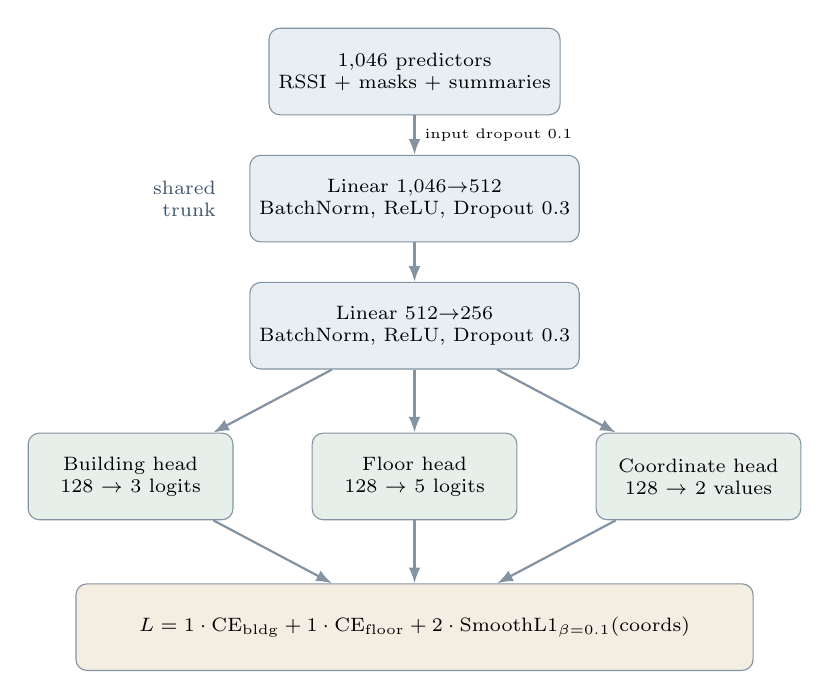
\begin{tikzpicture}[
  node distance=5mm and 6mm,
  pbox/.style={draw=SignalLine,rounded corners,align=center,minimum width=30mm,minimum height=11mm,fill=SignalBlue,font=\scriptsize},
  gbox/.style={draw=SignalLine,rounded corners,align=center,minimum width=26mm,minimum height=11mm,fill=SignalSage,font=\scriptsize},
  sbox/.style={draw=SignalLine,rounded corners,align=center,minimum width=26mm,minimum height=11mm,fill=SignalSand,font=\scriptsize},
  arrow/.style={-{Latex[length=2mm]},thick,draw=SignalLine}
]
\node[pbox] (in) {1,046 predictors\\RSSI $+$ masks $+$ summaries};
\node[pbox,below=of in] (t1) {Linear 1,046$\to$512\\BatchNorm, ReLU, Dropout 0.3};
\node[pbox,below=of t1] (t2) {Linear 512$\to$256\\BatchNorm, ReLU, Dropout 0.3};
\node[gbox,below left=8mm and 2mm of t2] (hb) {Building head\\128 $\to$ 3 logits};
\node[gbox,below=8mm of t2] (hf) {Floor head\\128 $\to$ 5 logits};
\node[gbox,below right=8mm and 2mm of t2] (hc) {Coordinate head\\128 $\to$ 2 values};
\node[sbox,below=8mm of hf,minimum width=86mm] (loss) {$L = 1\cdot\mathrm{CE}_{\mathrm{bldg}} + 1\cdot\mathrm{CE}_{\mathrm{floor}} + 2\cdot\mathrm{SmoothL1}_{\beta=0.1}(\mathrm{coords})$};
\draw[arrow] (in) -- node[right,font=\tiny]{input dropout 0.1} (t1);
\draw[arrow] (t1) -- (t2);
\draw[arrow] (t2) -- (hb);
\draw[arrow] (t2) -- (hf);
\draw[arrow] (t2) -- (hc);
\draw[arrow] (hb) -- (loss);
\draw[arrow] (hf) -- (loss);
\draw[arrow] (hc) -- (loss);
\node[left=3mm of t1,font=\scriptsize,text=SignalInk,align=right] {shared\\trunk};
\end{tikzpicture}%
}
\caption{Selected multitask network (768,906 parameters). All three heads read the same 256-unit trunk representation; the weighted loss combines the three tasks.}
\label{fig:architecture}
\end{figure}

\subsection{Loss}
The training loss is
\[
L = w_b\,\mathrm{CE}(\hat{y}_b, y_b) + w_f\,\mathrm{CE}(\hat{y}_f, y_f) + w_c\,\mathrm{SmoothL1}_{\beta}(\hat{\mathbf{c}}, \mathbf{c}),
\]
where CE is cross-entropy, $\mathbf{c}$ are standardized coordinates, and $\beta$ is the Smooth-L1 transition point. With $\beta=1$ the coordinate loss is quadratic for errors below one standard deviation, about 67--124 units, which gives fine position errors very small gradients. A preliminary internal-validation run with the 512--256 trunk gave selection scores of 0.0430 for $\beta=1$, 0.0355 for $\beta=0.1$, and 0.0378 for $\beta=0.02$, so $\beta=0.1$ is the default. A $\beta=1$ candidate stays in the selection grid so this choice is recorded with the other candidates.

\subsection{Training}
Training uses AdamW (learning rate $10^{-3}$, weight decay $10^{-4}$), batch size 256, and a learning rate halved when the validation score stops improving for 5 epochs. Training runs for at most 150 epochs and stops after 15 epochs without improvement, restoring the best weights. Python, NumPy, and PyTorch are seeded (seed 42) and PyTorch runs in deterministic mode. A full second run of the pipeline reproduced every reported metric exactly.

\subsection{Model selection}
Early stopping and the choice between candidates use one internal-validation score, where lower is better:
\[
S = \tfrac{1}{3}\left[(1-\mathrm{acc}_b) + (1-\mathrm{acc}_f) + \bar{e}/D\right].
\]
Here $\bar{e}$ is the mean Euclidean coordinate error and $D=125.9$ units is the internal-validation error of always predicting the internal-training centroid, which places the coordinate term on roughly the same 0--1 scale as the error rates. Ties go to the earlier, simpler candidate. Table~\ref{tab:selection} lists the seven candidates. The selected configuration and weights are written to disk before the held-out file is loaded.

\begin{table}[!t]
\centering
\caption{Multitask candidates on internal validation (3,852 records). Coordinate error in recorded units.}
\label{tab:selection}
\scriptsize
\setlength{\tabcolsep}{3pt}
\begin{tabular}{lcccrrr}
\toprule
Trunk & Drop. & $w_b/w_f/w_c$ & $\beta$ & Score & Floor & $\bar{e}$ \\
\midrule
\textbf{512--256} & \textbf{0.3} & \textbf{1/1/2} & \textbf{0.1} & \textbf{0.0346} & \textbf{97.87\%} & \textbf{10.28} \\
512--256 & 0.3 & 1/1/1 & 0.1 & 0.0355 & 97.79\% & 10.53 \\
1024--512--256 & 0.3 & 1/1/1 & 0.1 & 0.0360 & 97.98\% & 10.95 \\
512--256 & 0.3 & 1/2/1 & 0.1 & 0.0367 & 97.46\% & 10.56 \\
512--256 & 0.3 & 1/1/1 & 1.0 & 0.0375 & 97.85\% & 11.34 \\
1024--512 & 0.3 & 1/1/1 & 0.1 & 0.0438 & 97.69\% & 13.42 \\
512--256 & 0.5 & 1/1/1 & 0.1 & 0.0489 & 96.26\% & 13.65 \\
\bottomrule
\end{tabular}
\end{table}

The selected network stopped improving at epoch 25 and training ended at epoch 40; it takes about 40 seconds on a four-core CPU. Fig.~\ref{fig:history} shows its training curves.

\begin{figure}[!t]
  \centering
  \includegraphics[width=\columnwidth]{../results/figures/dl_05_multitask_training_history.png}
  \caption{Training loss terms and internal-validation selection score for the selected configuration. The marker shows the restored best epoch.}
  \label{fig:history}
\end{figure}

\subsection{Single-task ablations}
To isolate the effect of sharing the trunk, three networks of the same family are trained with a single head and loss term each, selecting among the four trunk candidates (512--256, 1024--512, 1024--512--256, and 512--256 with dropout 0.5) on their own internal-validation term. The selected trunks are 512--256 for building (all candidates tied at 99.95\%), 1024--512--256 for floor, and 1024--512 for coordinates. Combined, their predictions form a ``DL single-task'' comparison model; it has no joint building-floor accuracy because its two class predictions come from different networks.

\section{Evaluation measures}
Building and floor are scored with accuracy and macro-averaged F1. Coordinates are scored with the mean absolute error on each axis and with the per-record Euclidean error
\[
e_i = \sqrt{(\hat{x}_i-x_i)^2 + (\hat{y}_i-y_i)^2},
\]
summarized by its mean and median. Joint accuracy counts records where both building and floor are correct. All models are joined on (\texttt{SOURCE\_PARTITION}, \texttt{ROW\_ID}), so every comparison uses identical records.

Two paired tests check whether differences are real. For correctness, the exact McNemar test compares the records each model gets right and the other gets wrong. For coordinates, a bootstrap (2,000 resamples) gives a 95\% interval for the mean paired difference in Euclidean error. In addition, the frozen multitask configuration is retrained with seeds 7 and 2026, without re-selection, to show how much the held-out results vary with initialization.

Coordinate errors are reported in the dataset's recorded units. Phase 1 interpreted them as EPSG:3857 metres, but the repository contains no authoritative coordinate reference metadata, and EPSG:3857 units at this latitude overstate ground distance by roughly 1.3$\times$ even if that interpretation is right.

\section{Results}
\subsection{Held-out comparison}
Table~\ref{tab:results} compares the three models on the same 1,111 held-out records, and Fig.~\ref{fig:metric-comparison} shows the same values. The multitask network has the best building accuracy, floor accuracy, floor macro F1, and joint accuracy. The single-task coordinate network has the lowest coordinate errors. The Random Forest has the lowest median error, by a small margin.

\begin{table}[!t]
\centering
\caption{Held-out results on identical records. Coordinate errors in recorded units.}
\label{tab:results}
\small
\setlength{\tabcolsep}{4pt}
\begin{tabular}{lrrr}
\toprule
Metric & AML RF & DL multi & DL single \\
\midrule
Building accuracy & 99.73\% & \textbf{99.91\%} & 99.73\% \\
Building macro F1 & 99.71\% & \textbf{99.88\%} & 99.68\% \\
Floor accuracy & 88.93\% & \textbf{90.64\%} & 90.28\% \\
Floor macro F1 & 87.27\% & \textbf{89.35\%} & 89.17\% \\
Building and floor & 88.75\% & \textbf{90.64\%} & -- \\
Longitude MAE & 8.10 & 8.55 & \textbf{6.76} \\
Latitude MAE & 6.81 & 6.65 & \textbf{5.83} \\
Mean Euclidean & 11.58 & 11.88 & \textbf{9.84} \\
Median Euclidean & \textbf{7.49} & 9.80 & 7.59 \\
\bottomrule
\end{tabular}
\end{table}

\begin{figure}[!t]
  \centering
  \includegraphics[width=\columnwidth]{../results/figures/dl_05_multitask_heldout_metric_comparison.png}
  \caption{Held-out metrics for the three models. The left panel shows percentages and the right panel shows recorded coordinate units; heights should not be compared across panels.}
  \label{fig:metric-comparison}
\end{figure}

On internal validation, the multitask network reaches 99.92\% building accuracy, 97.87\% floor accuracy, and a mean coordinate error of 10.28; the baseline reaches 99.95\%, 96.42\%, and 8.58; the single-task networks reach 99.95\%, 98.18\%, and 7.68. All models lose accuracy on the held-out file, as expected from the partition differences described above.

\subsection{Are the differences real?}
Table~\ref{tab:paired} summarizes the paired tests on held-out records. The multitask network is right where the baseline is wrong on 37 floor predictions, and the reverse on 18 ($p=0.014$); for joint correctness the counts are 39 and 18 ($p=0.0075$). The building difference, 3 against 1 record, is not significant. For coordinates, the mean paired difference of $+0.30$ units has a 95\% interval that contains zero, and the multitask network is closer than the baseline on 39\% of records.

\begin{table}[!t]
\centering
\caption{Paired held-out comparison, DL multitask against AML RF.}
\label{tab:paired}
\small
\begin{tabular}{lccc}
\toprule
Task & DL only & AML only & Exact $p$ \\
\midrule
Building & 3 & 1 & 0.63 \\
Floor & 37 & 18 & 0.014 \\
Building and floor & 39 & 18 & 0.0075 \\
\midrule
\multicolumn{4}{l}{Coordinates: mean DL$-$AML $=+0.30$, 95\% CI $[-0.42, 1.02]$} \\
\bottomrule
\end{tabular}
\end{table}

Seed variation does not change these conclusions. With seeds 42, 7, and 2026, the frozen configuration reaches held-out floor accuracies of 90.64\%, 89.65\%, and 90.10\% (mean 90.13\%, standard deviation 0.50 percentage points), all above the baseline's 88.93\%. Mean coordinate errors are 11.88, 12.40, and 11.94 (mean 12.07, standard deviation 0.28), none below the baseline's 11.58. Building accuracy is 99.91\% for every seed.

\subsection{Floor classification}
Fig.~\ref{fig:floor-cm} compares the held-out floor confusion matrices, and Table~\ref{tab:floor-recall} gives per-floor recall. The multitask network improves recall on four of the five floors, with the largest gains on floor 4 (76.92\% against 69.23\%) and floor 2 (93.46\% against 91.18\%); recall on floor 0 falls slightly. As for the baseline, the most frequent error is true floor 1 predicted as floor 2, with 39 records against 49. Among records with the correct building, 97 of the 103 floor errors are off by exactly one floor.

\begin{figure}[!t]
  \centering
  \includegraphics[width=\columnwidth]{../results/figures/dl_05_multitask_heldout_floor_confusion_dl_vs_aml.png}
  \caption{Held-out floor confusion matrices for the DL multitask network (left) and the AML Random Forest (right). Rows are true floors.}
  \label{fig:floor-cm}
\end{figure}

\begin{table}[!t]
\centering
\caption{Held-out floor recall by true floor code.}
\label{tab:floor-recall}
\begin{tabular}{rrrr}
\toprule
True floor & Support & AML RF & DL multitask \\
\midrule
0 & 132 & 90.15\% & 88.64\% \\
1 & 462 & 86.80\% & 88.96\% \\
2 & 306 & 91.18\% & 93.46\% \\
3 & 172 & 94.19\% & 94.77\% \\
4 & 39 & 69.23\% & 76.92\% \\
\bottomrule
\end{tabular}
\end{table}

The improvement is concentrated in the cells that were hardest for the baseline. Floor accuracy for building 2, floor 2 rises from 68.5\% to 88.9\%; building 1, floor 1 from 65.7\% to 70.6\%; building 2, floor 4 from 69.2\% to 76.9\%. Building 1, floor 1 remains the weakest cell for both models.

\subsection{Coordinate errors}
Fig.~\ref{fig:error-map} maps held-out coordinate error at each true position, and Fig.~\ref{fig:error-dist} compares the error distributions. Large errors appear at scattered positions rather than as a uniform offset. The two models have differently shaped error distributions. The baseline places more records very precisely: 32.8\% of its errors are below 5 units, against 18.3\% for the multitask network, which explains its lower median. The multitask network has a much lighter tail: its 95th percentile is 28.24 units against 36.21, and its largest error is 66.6 against 135.1. These two effects roughly cancel in the mean. The multitask network's errors are also spread evenly across buildings (mean 11.47, 12.01, and 12.54 units for buildings 0, 1, and 2), whereas the baseline is far more precise in building 0 (7.97) than in buildings 1 and 2 (14.60 and 15.35).

\begin{figure}[!t]
  \centering
  \includegraphics[width=\columnwidth]{../results/figures/dl_05_multitask_heldout_error_map.png}
  \caption{Held-out coordinate error for the DL multitask network. Left: true positions coloured by Euclidean error (capped at the 95th percentile). Right: displacement from true to predicted position for 500 sampled records.}
  \label{fig:error-map}
\end{figure}

\begin{figure}[!t]
  \centering
  \includegraphics[width=\columnwidth]{../results/figures/dl_05_multitask_heldout_error_distribution_dl_vs_aml.png}
  \caption{Held-out Euclidean error distributions for the DL multitask network and the AML Random Forest: histogram (left) and cumulative share of records (right).}
  \label{fig:error-dist}
\end{figure}

\subsection{Hierarchical error analysis}\label{sec:hier}
Table~\ref{tab:hierarchy} groups held-out records by whether building and floor are correct, and Fig.~\ref{fig:hierarchy} shows the same breakdown. The multitask network has 21 more records with both building and floor correct, 19 fewer with only the floor wrong, and none with the wrong building but the right floor. When the floor is wrong, the baseline's coordinate error more than doubles (10.00 to 23.27 units), whereas the multitask network's rises less (11.27 to 17.88). Its coordinate prediction appears to stay coherent with its floor prediction, which is consistent with the shared representation. When both building and floor are correct, the baseline places records more precisely.

\begin{table}[!t]
\centering
\caption{Held-out records and mean coordinate error by building-floor outcome.}
\label{tab:hierarchy}
\small
\setlength{\tabcolsep}{4pt}
\begin{tabular}{lrrrr}
\toprule
& \multicolumn{2}{c}{AML RF} & \multicolumn{2}{c}{DL multitask} \\
Outcome & Rows & $\bar{e}$ & Rows & $\bar{e}$ \\
\midrule
Both correct & 986 & 10.00 & 1,007 & 11.27 \\
Building right, floor wrong & 122 & 23.27 & 103 & 17.88 \\
Building wrong, floor right & 2 & 44.31 & 0 & -- \\
Both wrong & 1 & 77.04 & 1 & 11.74 \\
\bottomrule
\end{tabular}
\end{table}

\begin{figure}[!t]
  \centering
  \includegraphics[width=\columnwidth]{../results/figures/dl_05_multitask_hierarchical_dl_vs_aml.png}
  \caption{Held-out records (log scale, left) and mean coordinate error (right) per building-floor outcome, DL multitask against AML RF.}
  \label{fig:hierarchy}
\end{figure}

\subsection{Robustness by phone}
Fig.~\ref{fig:phones} breaks held-out results down by \texttt{PHONEID}, after the fact; identifiers are never model inputs. Phone 13, which also appears in training and contributes 369 records, reaches 93.5\% floor accuracy. The nine unseen phones range from 76.5\% (phone 5, 17 records) to 95.0\% (phone 21, 60 records); the largest unseen group, phone 20 with 213 records, reaches 90.1\%. Group sizes are small and each phone's records come from particular times and places, so these differences are descriptive, not causal device effects. No user-level held-out analysis is possible because held-out \texttt{USERID} is a placeholder.

\begin{figure}[!t]
  \centering
  \includegraphics[width=\columnwidth]{../results/figures/dl_05_multitask_heldout_robustness_by_phone.png}
  \caption{Held-out floor accuracy and mean coordinate error by phone for the DL multitask network. Blue: phones also present in internal training.}
  \label{fig:phones}
\end{figure}

\section{Discussion}
The three targets respond differently to sharing. Building prediction is at its ceiling for every model, so it is not informative. Floor prediction benefits: both DL models beat the baseline, and the multitask network is slightly ahead of the floor-only network while using a smaller trunk. Coordinate regression suffers: the coordinate-only network is clearly the best regressor, while the multitask head, even with its loss weighted twice, is no better than the Random Forest. The likely cause is competition for the shared 256-unit representation, which the selection score rewards mainly for separating floors.

In practice, the multitask network is the better choice when one model must return building, floor, and position together, and especially when the floor matters most. When coordinate precision matters most, the single-task coordinate network should be used, or combined with the multitask classifier.

\section{Limitations}
\begin{itemize}
  \item \textbf{Partition scope:} results describe the supplied UJIIndoorLoc partition. It tests a later collection campaign with mostly unseen phones in the same buildings, not unseen buildings.
  \item \textbf{Coordinate reference:} coordinate errors are in recorded units. The coordinate reference system is not verified and no scale correction is applied.
  \item \textbf{Model search:} the grids are small (seven multitask and four single-task candidates per task) so they run on a CPU. Selection uses one seed on one internal split; the seed study covers only the frozen configuration.
  \item \textbf{Optimistic validation:} internal validation shares users, phones, period, some fingerprints, and many positions with training, which favors fitting the training campaign and partly explains the gap to held-out scores.
  \item \textbf{No hierarchy constraint:} building and floor heads are independent, and the coordinate head is not restricted to the predicted building's area.
  \item \textbf{Specification access:} the project specification document was not available in the environment that produced the implementation; the design follows its stated requirements.
\end{itemize}

\section{Team contributions}
The implementation was delivered as six dependency-ordered pull requests, each closing one GitHub issue. Krishiv wrote the project documentation, contributing guide, and package foundation, and later the multitask evaluation, AML comparison, and documentation. Gargi delivered the data layer and the data preparation notebook. Bhawana delivered the metrics, error analysis, and plotting layer. Agrima delivered the multitask network and training loop. Abhiman delivered the pipeline runner and the three single-task ablation notebooks. All five reviewed the final documentation and results.

\section{Conclusion}
A shared-trunk multitask network trained on the Phase 1 features and split improves held-out floor accuracy from 88.93\% to 90.64\% and joint building-and-floor accuracy from 88.75\% to 90.64\%; the floor gain is significant and stable across seeds. Its coordinate error is no better than the Random Forest's, while a dedicated coordinate network lowers mean error to 9.84 recorded units. Sharing a representation therefore helps the classification tasks and costs position accuracy. The code, saved models, notebooks, and result tables in the project repository reproduce every number in this paper.

\small
\begin{thebibliography}{9}
\bibitem{dawes2011}
B. Dawes and K.-W. Chin, ``A comparison of deterministic and probabilistic methods for indoor localization,'' \emph{Journal of Systems and Software}, vol. 84, no. 3, pp. 442--451, Mar. 2011, doi: \href{https://doi.org/10.1016/j.jss.2010.11.888}{10.1016/j.jss.2010.11.888}.

\bibitem{hechan2016}
S. He and S.-H. G. Chan, ``Wi-Fi fingerprint-based indoor positioning: Recent advances and comparisons,'' \emph{IEEE Communications Surveys \& Tutorials}, vol. 18, no. 1, pp. 466--490, 1st Quart. 2016, doi: \href{https://doi.org/10.1109/COMST.2015.2464084}{10.1109/COMST.2015.2464084}.

\bibitem{song2019}
X. Song, X. Fan, C. Xiang, Q. Ye, L. Liu, Z. Wang, X. He, and G. Fang, ``A novel convolutional neural network based indoor localization framework with WiFi fingerprinting,'' \emph{IEEE Access}, vol. 7, pp. 110698--110709, 2019, doi: \href{https://doi.org/10.1109/ACCESS.2019.2933921}{10.1109/ACCESS.2019.2933921}.

\bibitem{torres2014}
J. Torres-Sospedra, R. Montoliu, A. Mart\'{i}nez-Us\'{o}, J. P. Avariento, T. J. Arnau, M. Benedito-Bordonau, and J. Huerta,
``UJIIndoorLoc: A new multi-building and multi-floor database for WLAN fingerprint-based indoor localization problems,''
in \emph{Proc. 2014 International Conference on Indoor Positioning and Indoor Navigation (IPIN)}, Busan, Republic of Korea, 2014, pp. 261--270, doi: \href{https://doi.org/10.1109/IPIN.2014.7275492}{10.1109/IPIN.2014.7275492}.

\bibitem{uci}
UCI Machine Learning Repository, ``UJIIndoorLoc,'' dataset 310, doi: \href{https://doi.org/10.24432/C5MS59}{10.24432/C5MS59}. Available: \url{https://archive.ics.uci.edu/dataset/310/ujiindoorloc}.

\bibitem{breiman2001}
L. Breiman, ``Random forests,'' \emph{Machine Learning}, vol. 45, pp. 5--32, 2001, doi: \href{https://doi.org/10.1023/A:1010933404324}{10.1023/A:1010933404324}.

\bibitem{caruana1997}
R. Caruana, ``Multitask learning,'' \emph{Machine Learning}, vol. 28, pp. 41--75, 1997, doi: \href{https://doi.org/10.1023/A:1007379606734}{10.1023/A:1007379606734}.
\end{thebibliography}

\end{document}
